\chapter{Resultate und Testen} \label{chap:resultate}

\section{Testen} \label{sec:testen}

Die Webseite lässt in einer lokalen Entwicklungsumgebung oder auf der
öffentlichen Seite testen. Getestet wurden die Funktionen manuell von Hand oder
auch teilweise durch automatisierte Tests.

Grundsätzlich funktionieren alle Funktionen. Schlussendlich gibt es nur ein
Problem: Es kommt vor, dass der Webscraper Edge-Cases antrifft. Das kann
passieren, wenn die offizielle Mensa Webseite die Informationen auf ihrer
Webseite kurzfristig ändern. Es wurde versucht diese Edge-Cases möglichst alle
abzufangen, allerdings kann es immer noch sein, dass es manchmal zu Fehlern
kommt und die Daten der Webseite sich von der offiziellen Webseite
unterscheiden. Diese Fehler müssen jeweils von einem Admin auf der Admin-Seite
behoben werden.

\section{Resultate} \label{sec:resultate}

Das Resultat dieser Webseite ist eine voll Funktionstüchtige Webseite
Die Webseite erfüllt alle nötigen Anforderungen (siehe
\ref{sec:problemdefinition}). Die Webseite ist auch öffentlich zugänglich
(siehe \ref{spez:Deployment}) und kann unter
\url{http://mensarating.herokuapp.com/} aufgerufen werden. 
\subsection{Resultate der Grundanforderungen}
 
\newpage

\subsubsection*{Anzeige der Menus}

\begin{figure}[ht]
    \centering
    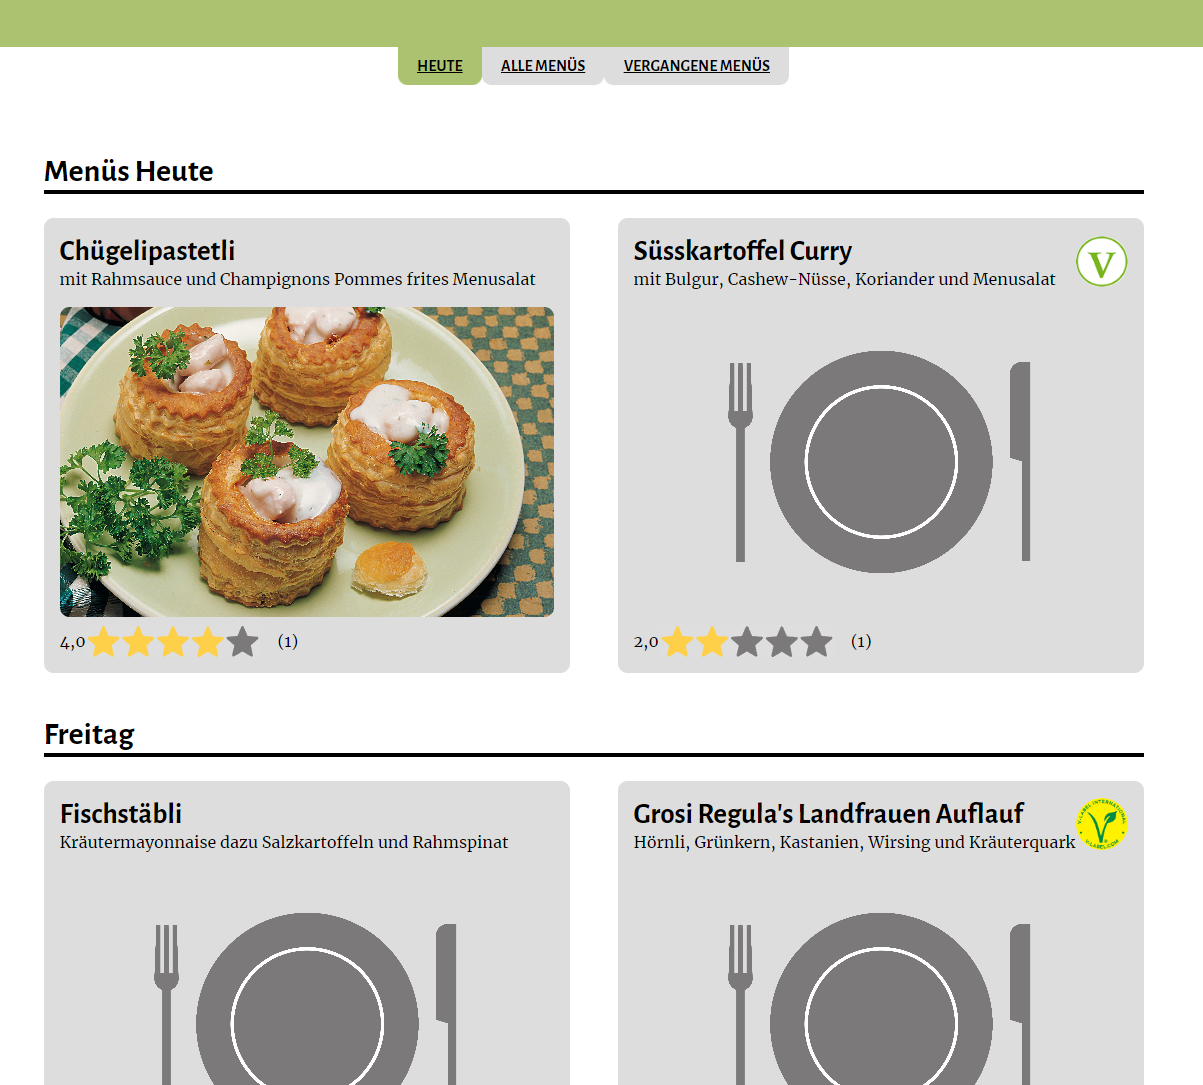
\includegraphics[width=0.8\textwidth]{images/Resultate_Menu.png}
    \caption{Screenshot: Anzeige Menus auf Startseite}
    \label{fig:r-menuindex}
\end{figure}

Auf der Startseite der Webseite (siehe \ref{fig:r-menuindex}) werden die beiden Menus des Tages, die von der
offiziellen Mensa Webseite gescraped wurden, angezeigt. Es wird die
Beschreibung, ein Label (Vegan/Vegetarisch), das durchschnittliche Rating und
das Bild mit den meisten Likes angezeigt. Als Zusatz sind die zukünftigen Menus
ebenfalls angezeigt.

\begin{figure}[htp]
    \begin{subfigure}[b]{0.5\textwidth}
        \centering
        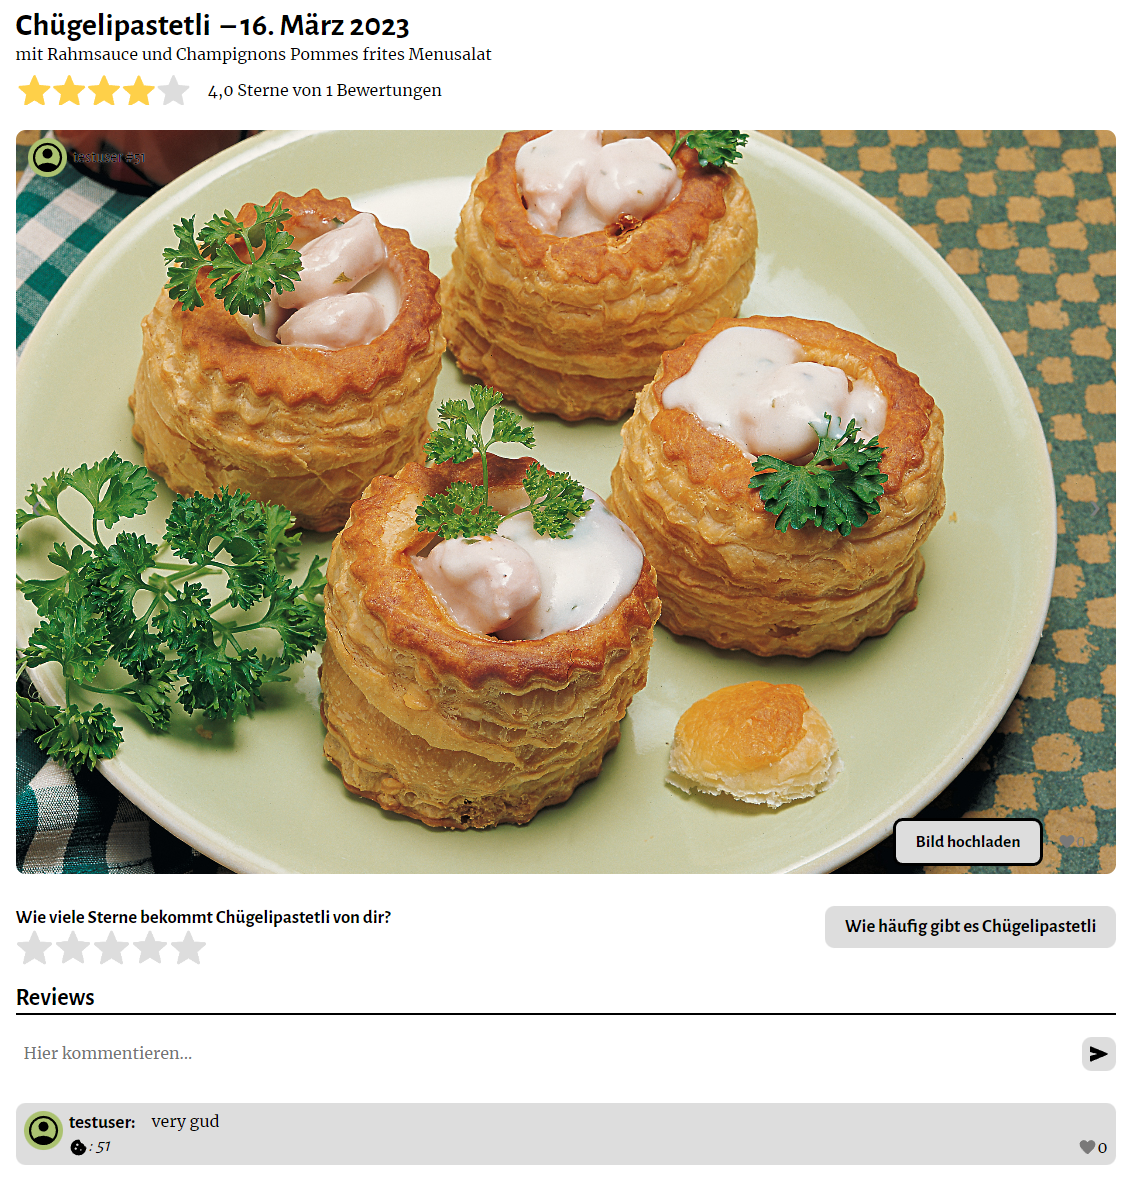
\includegraphics[width=0.7\textwidth]{images/Res_Menu.png}
        \caption{Screenshot: Menu Web Page}
        \label{fig:r-menu}
    \end{subfigure}
    \begin{subfigure}[b]{0.5\textwidth}
        \centering
        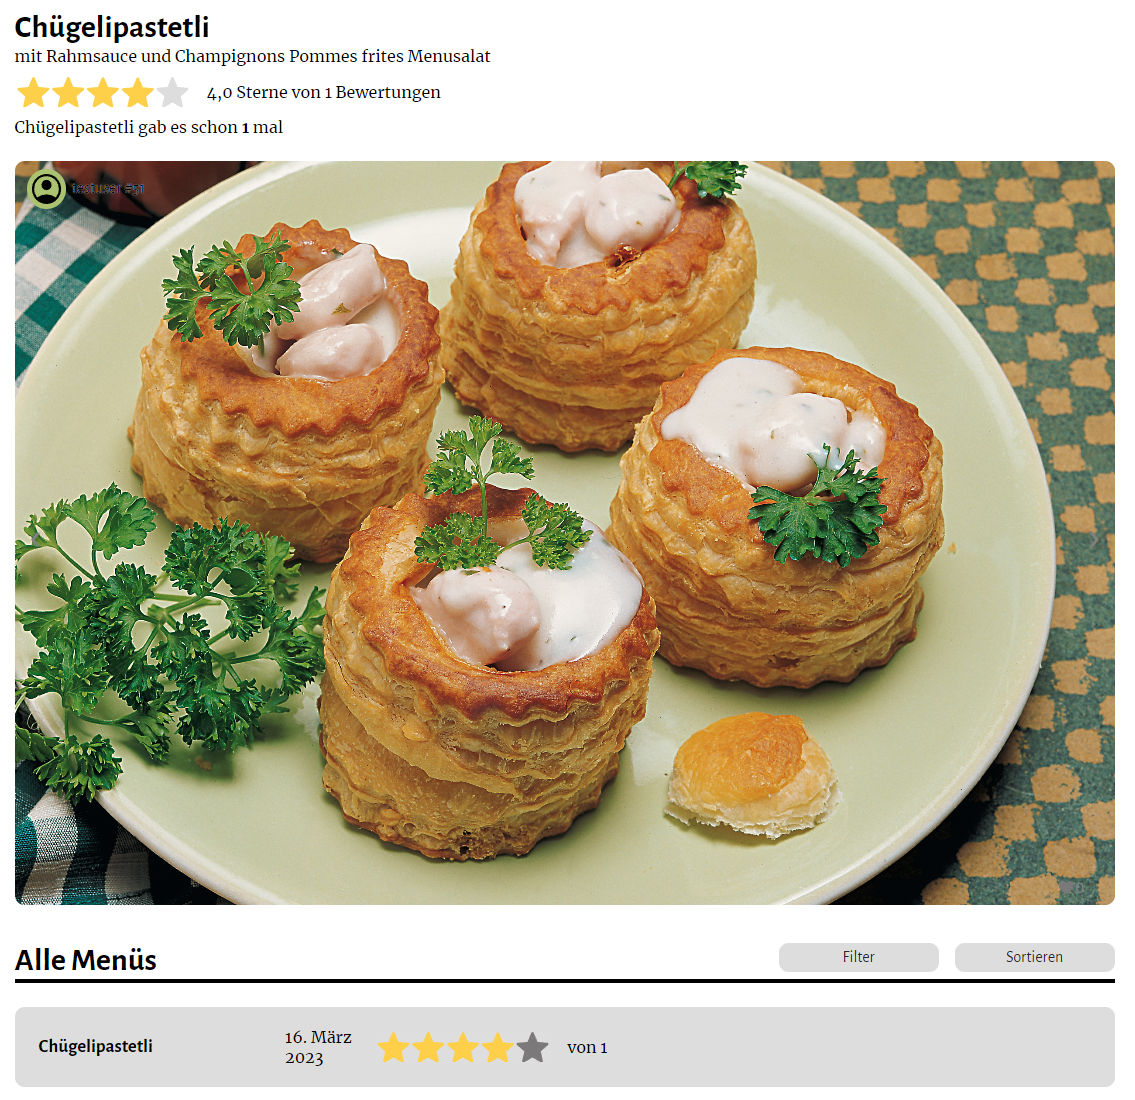
\includegraphics[width=0.7\textwidth]{images/Res_Menutype.png}
        \caption{Screenshot: Menutype Web Page}
        \label{fig:r-menutype}
    \end{subfigure}
    \hfill
\end{figure}

Zusätzlich gibt es eine Menu Page (siehe \ref{fig:r-menu}) und eine MenuType
Page (siehe \ref{fig:r-menutype}), wo die Menus genauer angezeigt werden  


\subsubsection*{Bilder Gallerie}

\begin{figure}[htp]
    \begin{subfigure}[b]{0.5\textwidth}
        \centering
        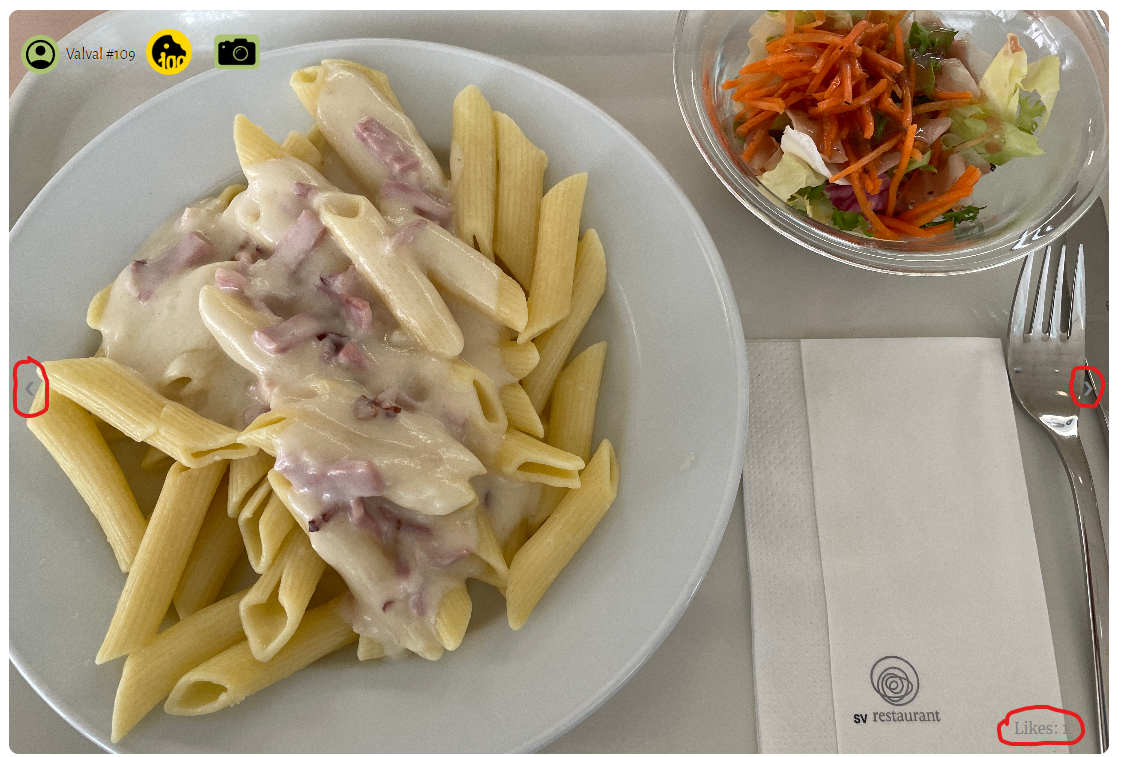
\includegraphics[width=0.7\textwidth]{images/Resultate_Bildergallerie.png}
        \caption{Screenshot: Bildergallerie}
        \label{fig:r-bildergallerie}
    \end{subfigure}
    \begin{subfigure}[b]{0.5\textwidth}
        \centering
        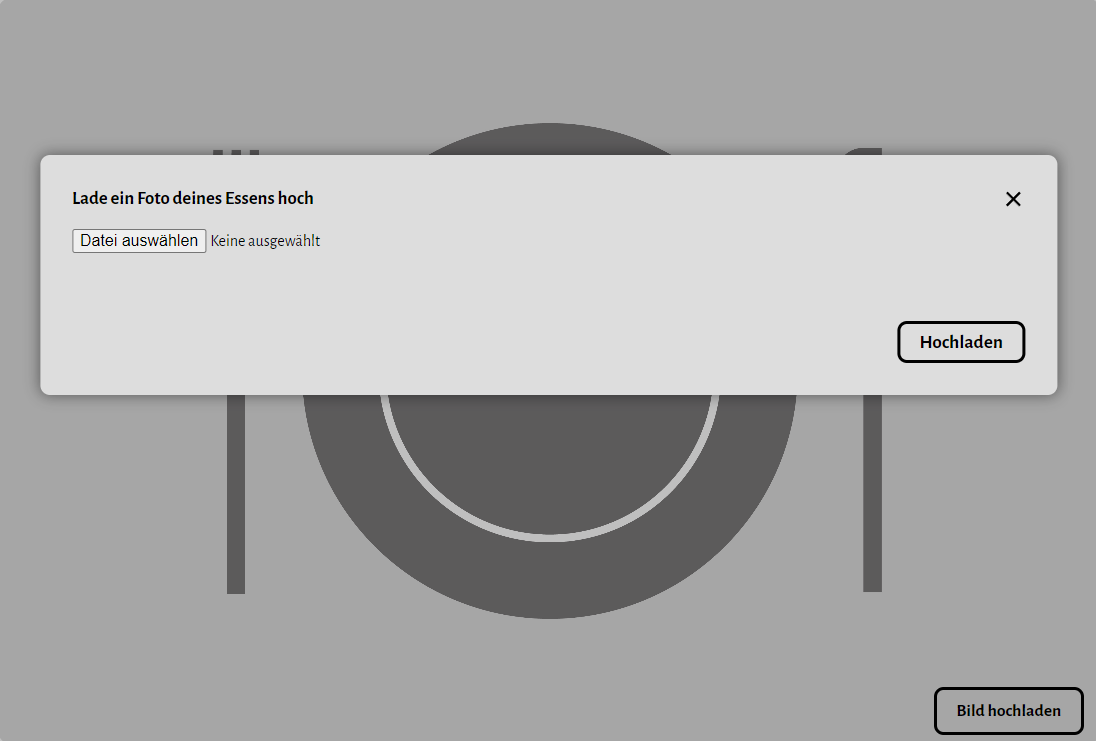
\includegraphics[width=0.7\textwidth]{images/Resultat_Bildergallerie_upload.png}
        \caption{Screenshot: Bilder Upload}
        \label{fig:r-bildpopup}
    \end{subfigure}
    \hfill
\end{figure}

Bei der Bildergallerie (siehe \ref{fig:r-bildergallerie}) können User Bilder
hochladen. Man kann durch Pfeil-Buttons die verschiedenen hochgeladenen Bilder
ansehen. Für jedes Bild ist erstens der User angezeigt, der es hochgeladen hat, und zweitens die
Anzahl Likes. Der Upload findet über einen Upload Button statt, der ein Pop-Up
öffnet (siehe \ref{fig:r-bildpopup})


\subsubsection*{Reviews}

\begin{figure}[ht]
    \centering
    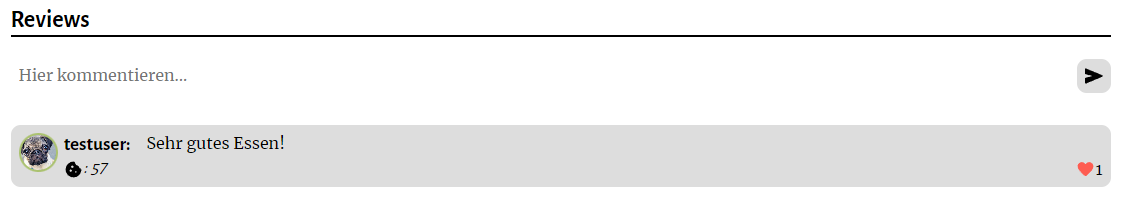
\includegraphics[width=0.8\textwidth]{images/Resultat_Review.png}
    \caption{Screenshot: Veröffentlichung und Anzeige von Reviews}
    \label{fig:r-review}
\end{figure}

Am Tag, an dem es ein bestimmtes Menu gibt, kann diesem Menu ein Review (siehe
\ref{fig:r-review}) gegeben werden. Die Reviews sind in einer Liste angeordet
und bei jedem Review ist der User angegeben, zusammen mit seinen Achievements
und Karma Punkten. Reviews können geliked werden (beachte das Herz).

\subsubsection*{Rating}

\begin{figure}[ht]
    \centering
    
\includegraphics[width=0.8\textwidth]{images/Resultat_Rating.png}
    \caption{Screenshot: Anzeige vom Rating eines Menus}
    \label{fig:r-rating}
\end{figure}

Ein User kann einem Menu als Rating einen bis fünf Sterne gebe. Der User drückt
dabei auf die Anzahl Sterne, die er geben will. Der Durchschnitt des Ratings
wird ebenfalls in der Form von Sternen angezeigt. Dabei kann es auch nicht volle
Sterne geben (siehe \ref{fig:r-rating}) 

\subsubsection*{Filtern/Sortieren}

\begin{figure}[ht]
    \centering
    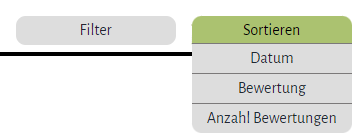
\includegraphics[width=0.8\textwidth]{images/Resultat_Filter.png}
    \caption{Screenshot: Buttons für Filter- und Sortier-Optionen}
    \label{fig:r-filtersort}
\end{figure}

auf der `Alle Menüs' Page und der `MenuType' Page können die Menüs/MenuTypes
nach verschiedenen Optionen in einem Dropdown-Menu (siehe
\ref{fig:r-filtersort}) gefiltert/sortiert werden. Nach der Auswahl wird die
Aktion ohne einen Reload der Seite ausgeführt.

\subsubsection*{Design}
Das Design ist an allen bisherigen Screenshots erkennbar. Als Akzentfarbe wurde
ein Grün gewählt, an vielen Formen sind die Ecken abgerundet und die
verschiedenen Aktionen auf der Webseite sollten für den User so einfach wie
möglich gestaltet sein.

\newpage

\subsection{Resultate der Erweiterungskriterien}

\subsubsection*{Account System}

\begin{figure}[htp]
    \begin{subfigure}[b]{0.32\textwidth}
        \centering
        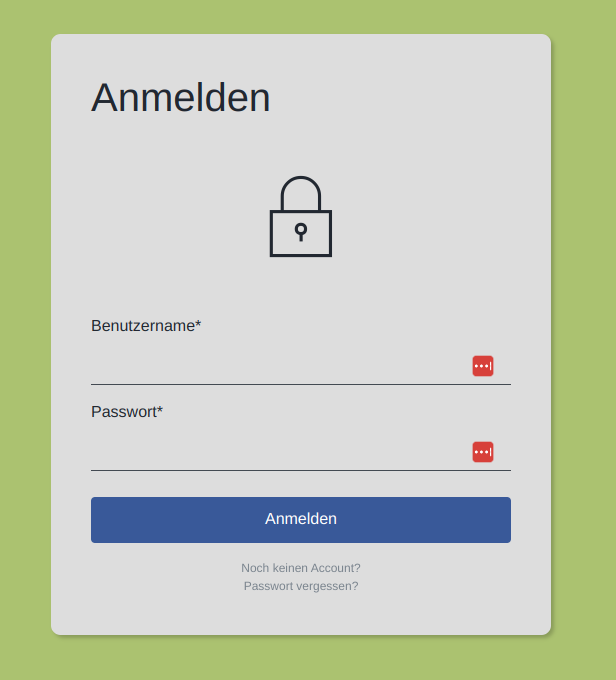
\includegraphics[width=0.7\textwidth]{images/Auth1.png}
        \caption{Screenshot: Login Form}
        \label{fig:r-login}
    \end{subfigure}
    \begin{subfigure}[b]{0.32\textwidth}
        \centering
        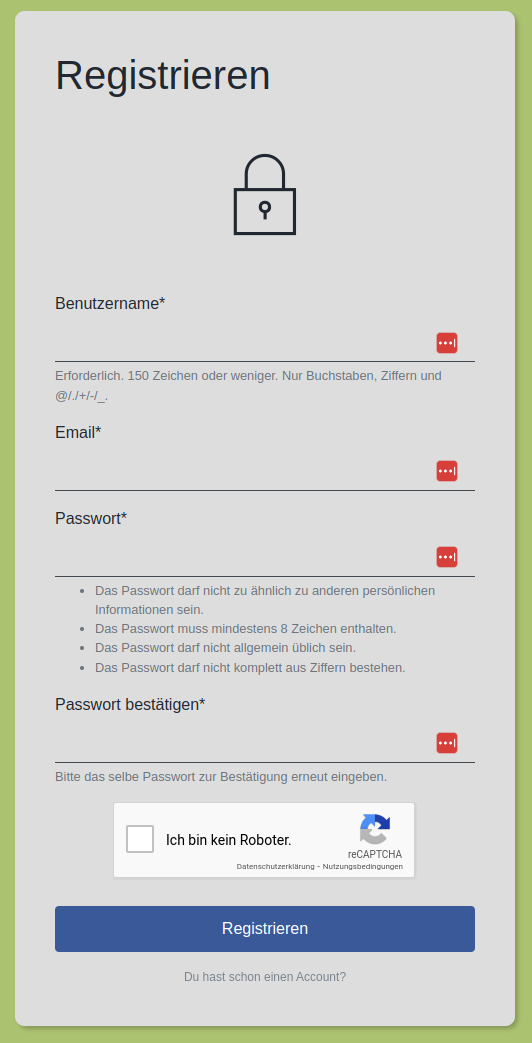
\includegraphics[width=0.5\textwidth]{images/Auth2.png}
        \caption{Screenshot: Registrieren Form}
        \label{fig:r-register}
    \end{subfigure}
    \begin{subfigure}[b]{0.32\textwidth}
        \centering
        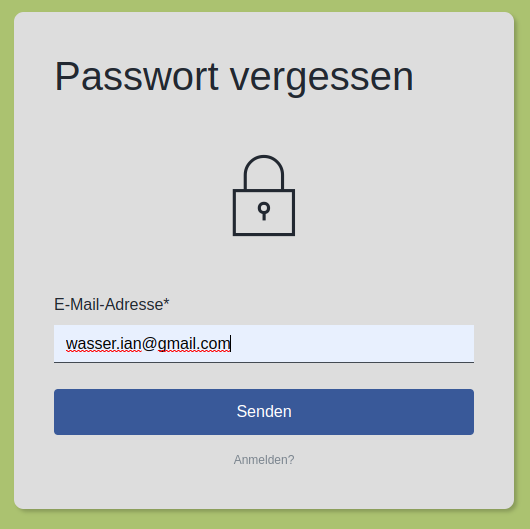
\includegraphics[width=0.7\textwidth]{images/Auth3.png}
        \caption{Screenshot: Passwort Reset Form}
        \label{fig:r-reset}
    \end{subfigure}
    \begin{subfigure}[b]{\textwidth}
        \centering
        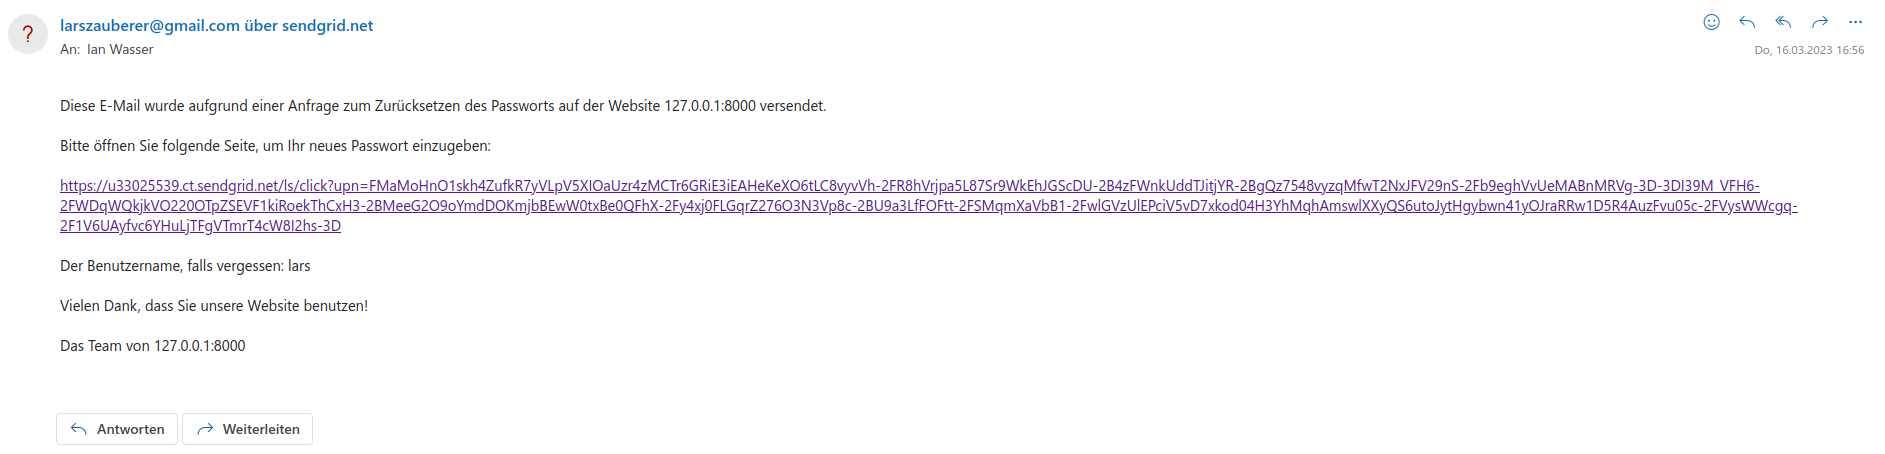
\includegraphics[width=\textwidth]{images/Auth4.png}
        \caption{Screenshot: Passwort Reset Mail}
        \label{fig:r-reset-mail}
    \end{subfigure}
    \begin{subfigure}[b]{\textwidth}
        \centering
        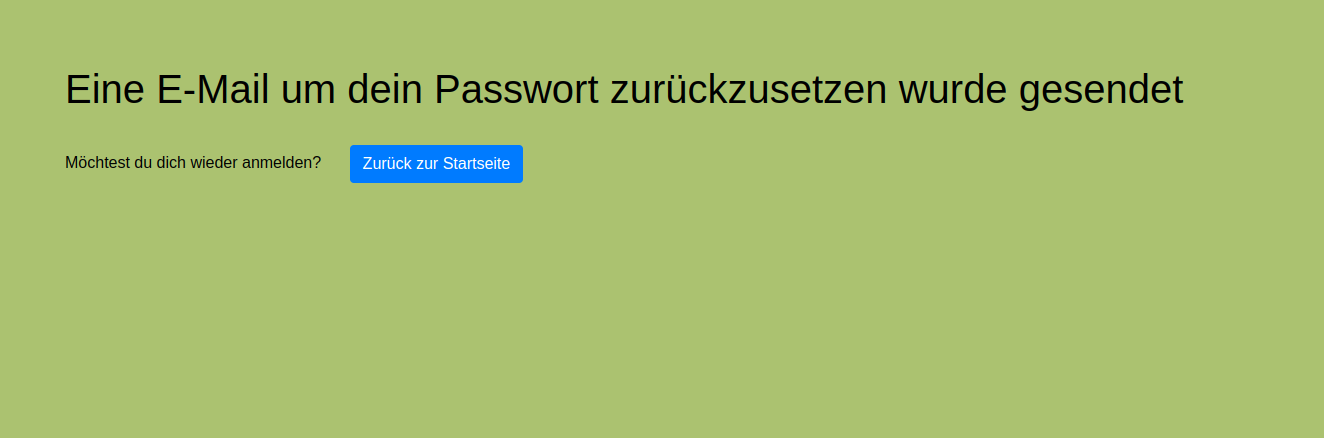
\includegraphics[width=\textwidth]{images/Auth5.png}
        \caption{Screenshot: Passwort Reset Complete}
        \label{fig:r-reset-complete}
    \end{subfigure}
    \caption{Screenshots: Account System}
    \label{fig:r-auth}
\end{figure} 

Die Webseite verfügt über ein komplett funktionierendes Account System. Wie den
einzelnen Screenshots zu entnehmen, kann der User sich registrieren, sich
einloggen, sich ausloggen und sein Passwort zurücksetzen.

\subsubsection*{Mobile Responsiveness}

\begin{figure}[ht]
    \centering
    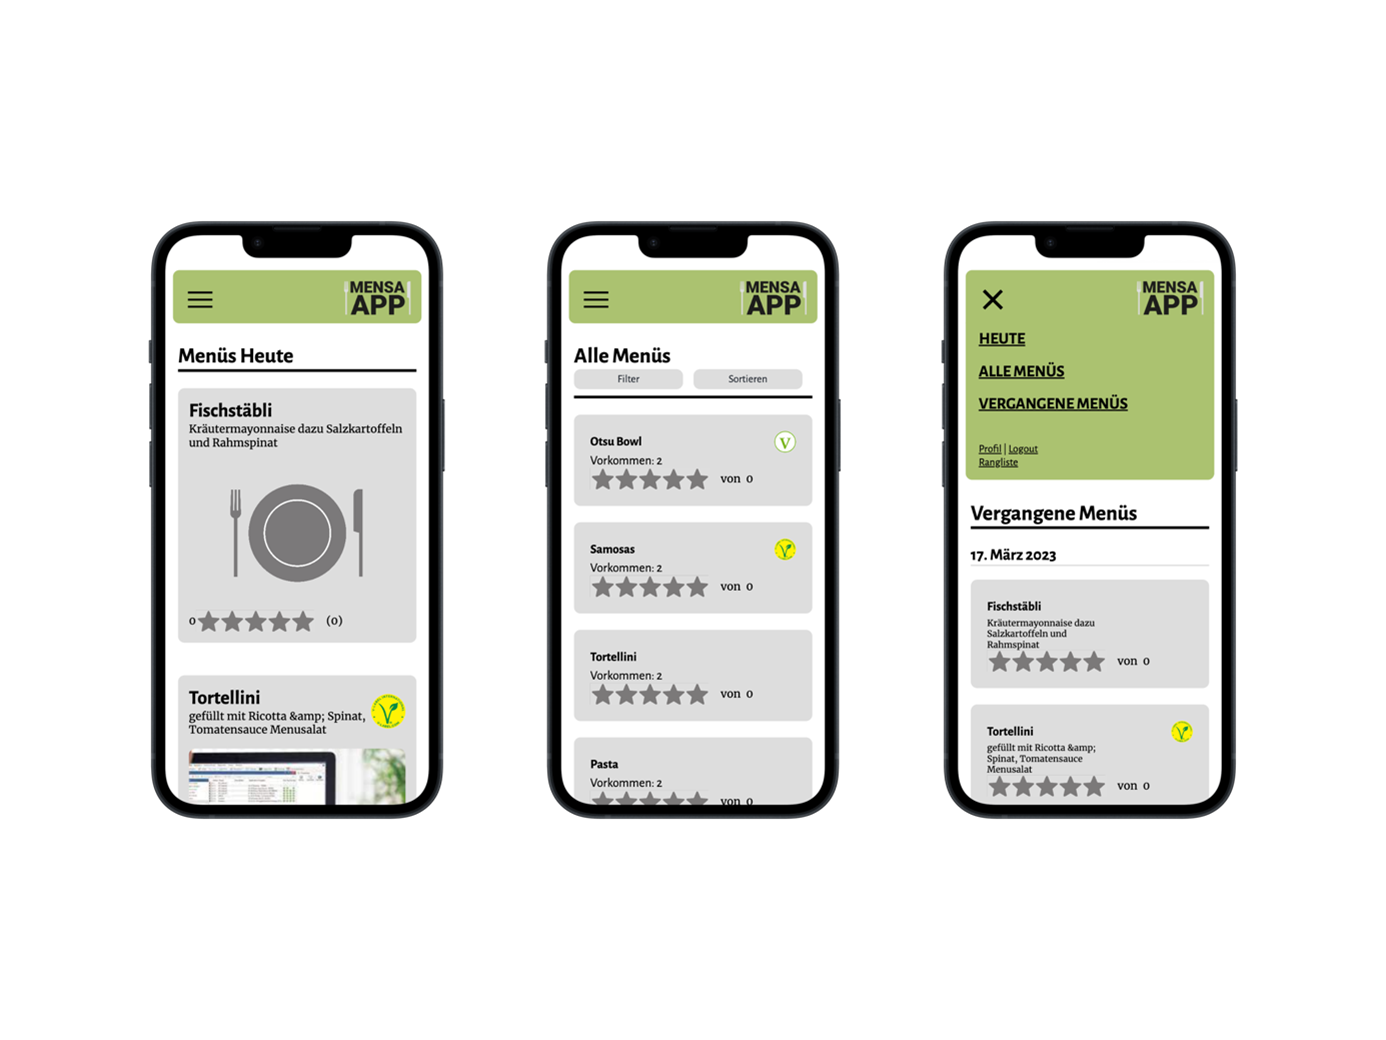
\includegraphics[width=0.8\textwidth]{images/Resultat_Responsive.png}
    \caption{Drei Beispiele der Mobile Responsiveness}
    \label{fig:r-karma}
\end{figure}

Beim Entwickeln der Website wurde davon ausgegangen, dass die meisten User mit
mobilen Endgeräten auf die Seite zugreifen. Daher ist es zentral, dass die
Website auf kleinen Bildschirmen einfach zu bedienen ist. Da ein Grossteil der
Seite mit Flexboxen designt wurde, war es meist einfach, den Inhalt für kleinere
Bildschirme anzupassen. Für andere Teile wurde ein komplett neues Design
erstellt, welches mithilfe von Media Queries nur auf kleinen Bildschirmen
dargestellt wird. Die Navigationselemente wurden komplett überarbeitet und
kleinere Seitenränder angewendet. Das Ziel, die Website Mobile Responsive zu
machen, wurde mit den oben erwähnten Schritten erreicht.


\subsubsection*{Punktesystem (Karma)}

\begin{figure}[ht]
    \centering
    
\includegraphics[width=0.5\textwidth]{images/Resultat_Karma.png}
    \caption{Screenshot: Karma eines Users (Auf Profilseite)}
    \label{fig:r-karma}
\end{figure}

User erhalten für Interaktionen auf der Webseite so genannte Cookiepoints (siehe
\ref{fig:r-karma}). Das Geben eines Ratings gibt einen Cookiepoint und das
Hochladen eines Bildes oder Reviews gibt 5 Cookiepoints. Wenn ein Post geliked
wird (siehe \ref{spez:Posts}), erhält der User, der geposted hat, einen
Cookiepoint. 

\begin{figure}[ht]
    \centering
    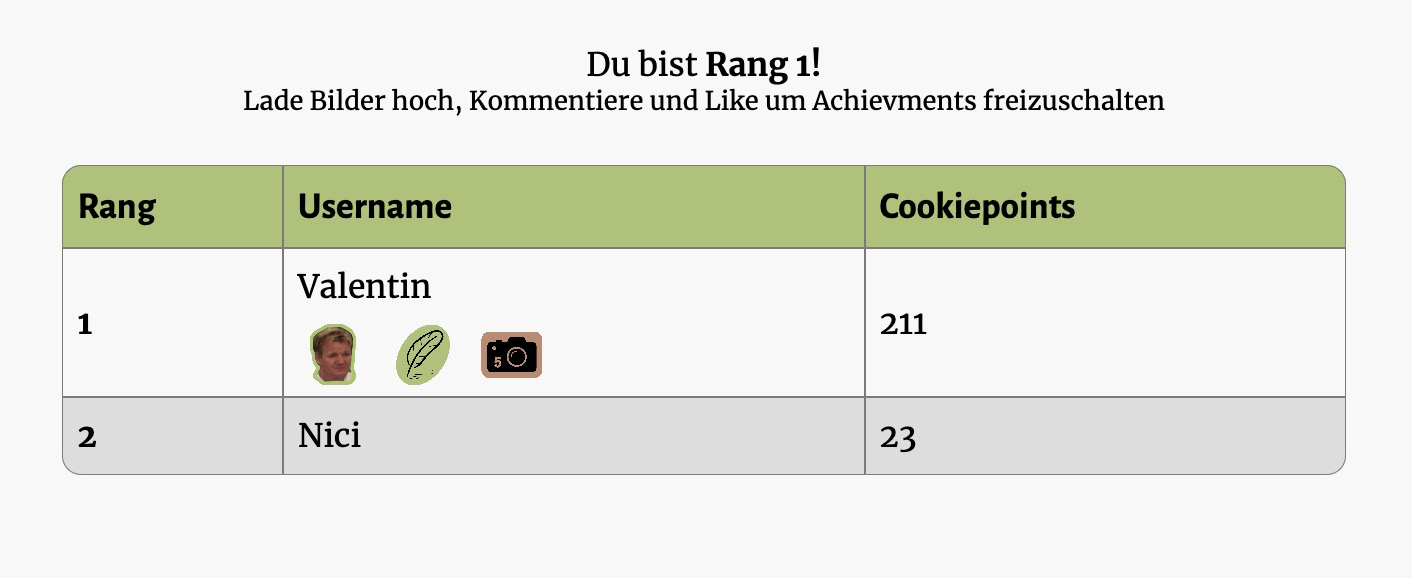
\includegraphics[width=0.8\textwidth]{images/Resultat_Rangliste.png}
    \caption{Screenshot: Karma Rangliste}
    \label{fig:r-rangliste}
\end{figure} 

Alle User mit Account sind in einer Rangliste aufgelistet. Die Rangliste bezieht
sich auf die Cookiepoints. Der User hat eine Angabe, wo er sich auf der
Rangliste befindet.

\subsubsection*{Achievement System}

\begin{figure}[ht]
    \centering
    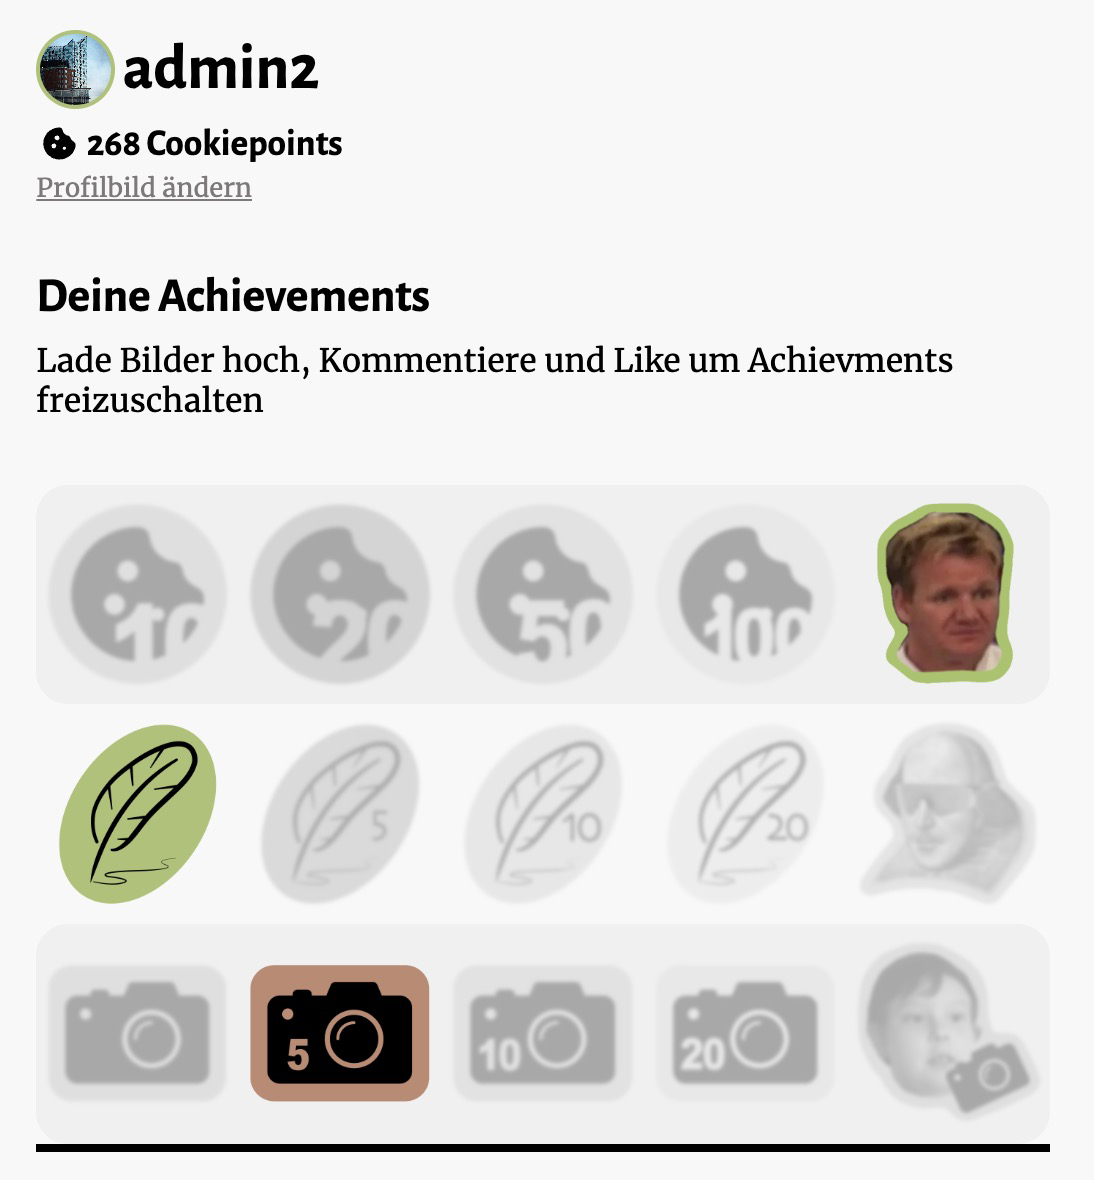
\includegraphics[width=0.8\textwidth]{images/Resultate_Achievements.png}
    \caption{Screenshot: Achievements Liste (Profil Page)}
    \label{fig:r-Achievement}
\end{figure} 

User können Achievements (siehe \ref{fig:r-Achievement}) erhalten. Die Bedinungen, um die Achievements zu
erhalten, sind in den Spezifikationen definiert (siehe \ref{spez:Badges}). Es
gibt fünf Achievements pro Kategorie. Wenn von einer Kategorie ein besseres
Achievement freigeschalten wird, wird dem User das Alte Achievement wieder
entzogen.

\begin{figure}[htp]
    \begin{subfigure}[b]{0.5\textwidth}
        \centering
        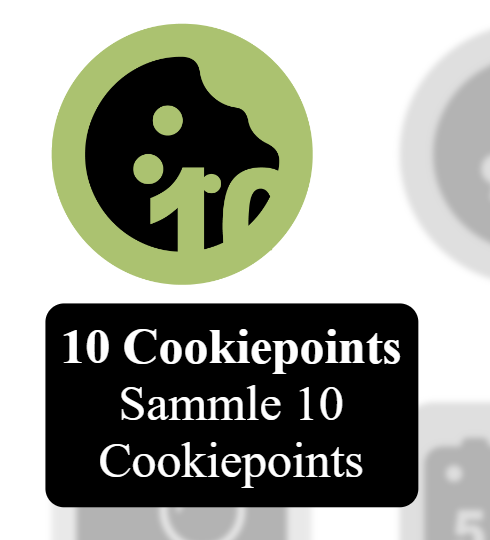
\includegraphics[width=0.7\textwidth]{images/Resultat-Beschreibung.png}
        \caption{Screenshot: Bildergallerie}
        \label{fig:r-Achievement-beschreibung}
    \end{subfigure}
    \begin{subfigure}[b]{0.5\textwidth}
        \centering
        
\includegraphics[width=0.7\textwidth]{images/Resultat-Username.png}
        \caption{Screenshot: Bilder Upload}
        \label{fig:r-username-display}
    \end{subfigure}
    \hfill
\end{figure}

Zu jedem Achievement gibt es eine kurze Beschreibung (siehe
\ref{fig:r-Achievement-beschreibung}), die angezeigt wird, wenn der User mit dem
Mauszeiger über dem Achievement hovered. Ausserdem werden die Achievements neben
dem User bei seinen Posts angezeigt (siehe \ref{fig:r-username-display}).

\newpage

\subsubsection*{Deployment}

\begin{figure}[ht]
    \centering
    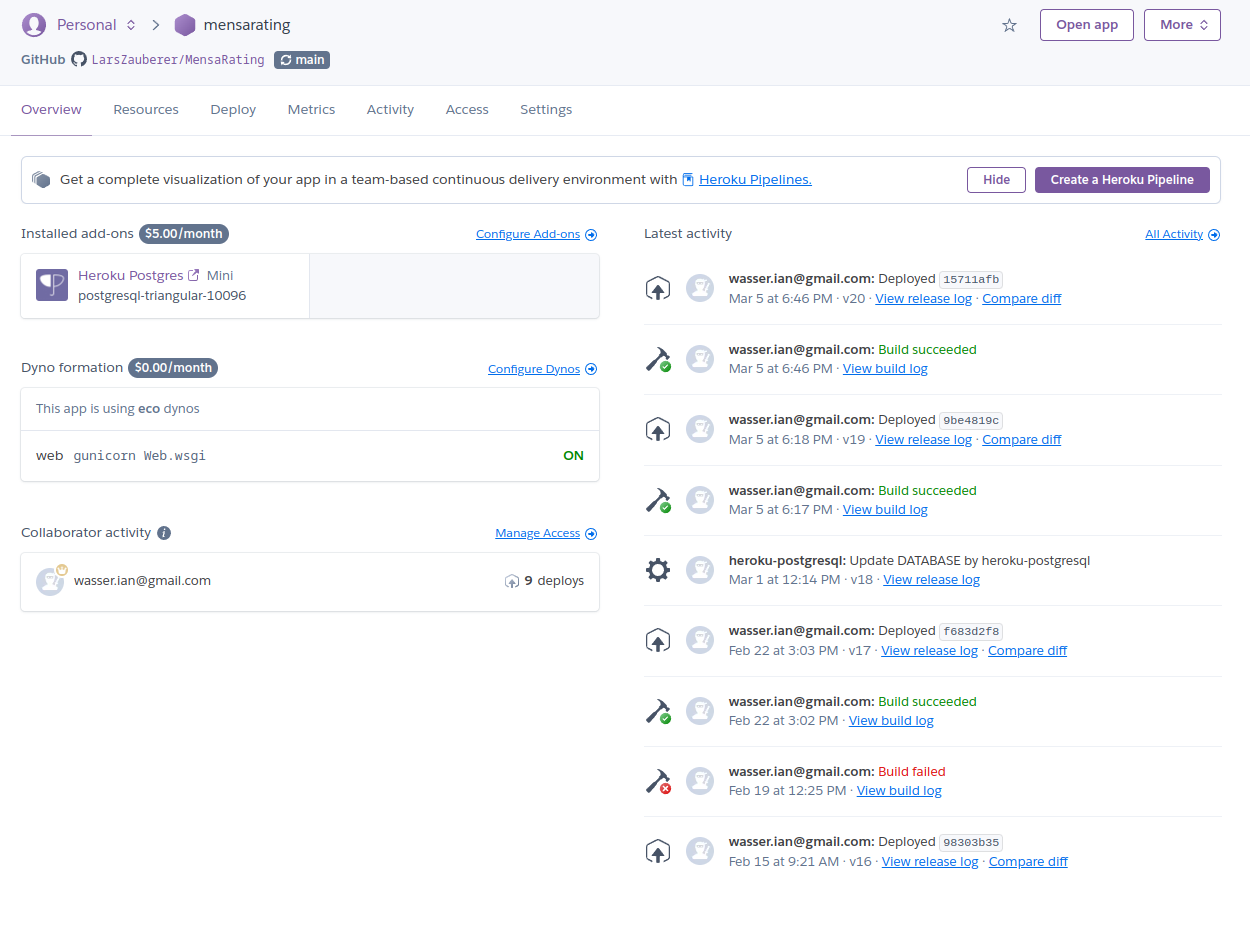
\includegraphics[width=0.8\textwidth]{images/Heroku.png}
    \caption{Screenshot: Heroku Interface für die App}
    \label{fig:r-deployment}
\end{figure}

Die Webseite wurde auf Heroku (siehe Interface der Heroku App
\ref{fig:r-deployment}) mit einem Eco-Server und einer Postgres Datenbank
veröffentlicht.

\newpage

\subsection{Datenbank}

\begin{figure}[ht]
    \centering
    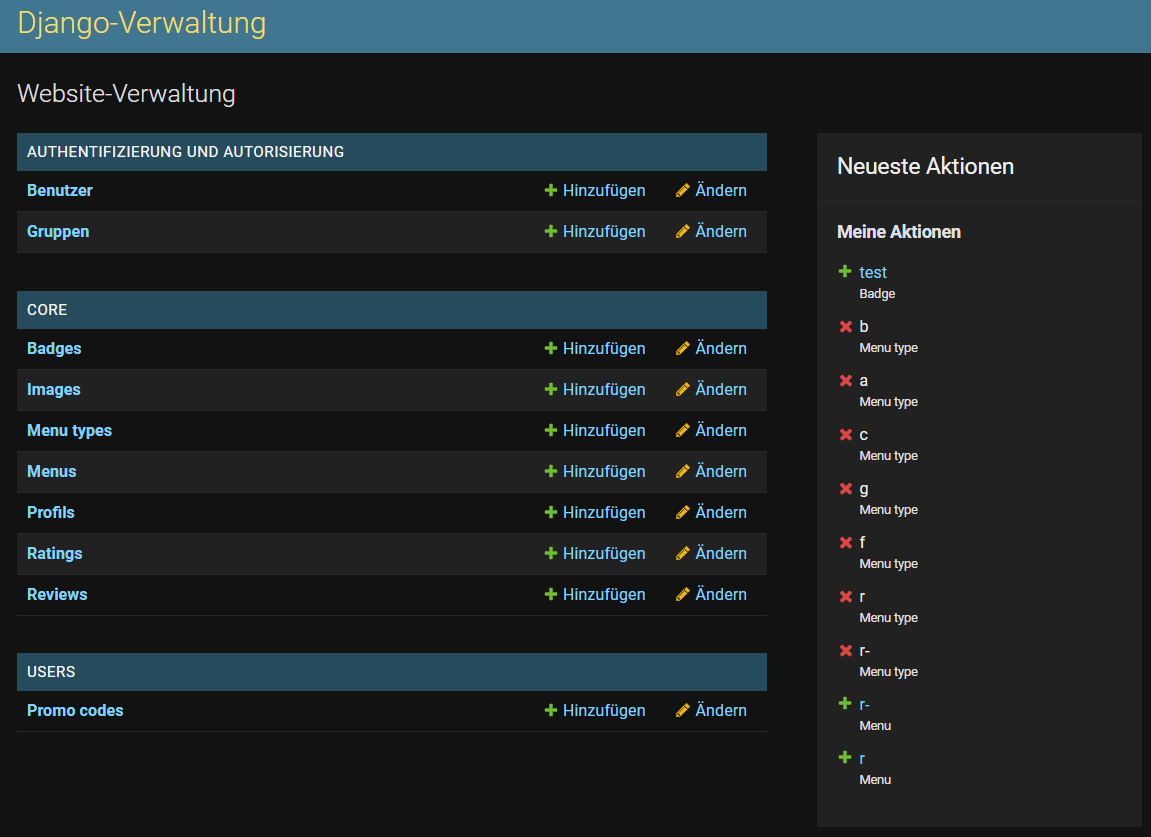
\includegraphics[width=0.8\textwidth]{images/Resultat-Adminpanel.png}
    \caption{Screenshot: Admin panel Web Page von Django}
    \label{fig:r-adminpanel}
\end{figure}

\begin{figure}[htp]
    \begin{subfigure}[b]{0.5\textwidth}
        \centering
        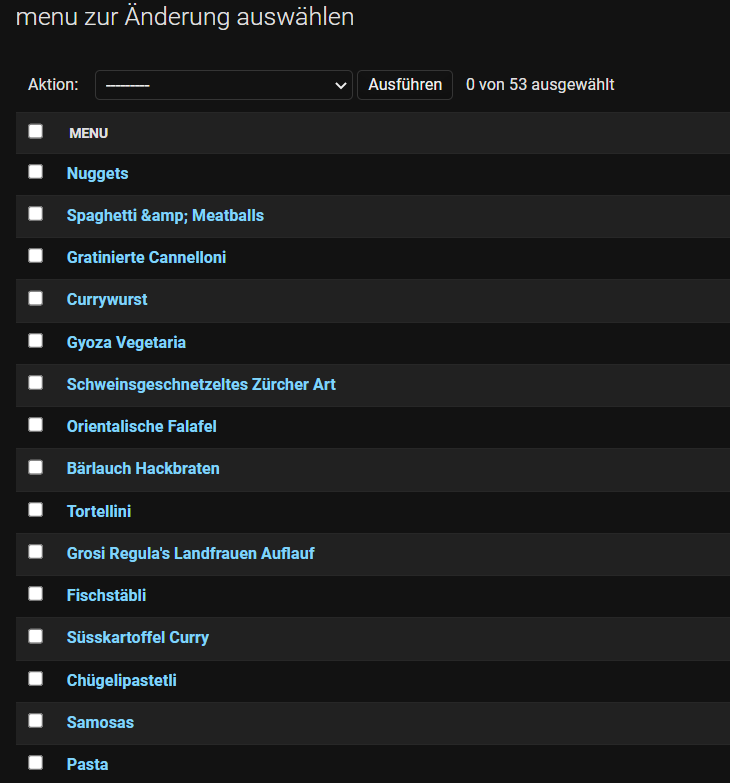
\includegraphics[width=0.7\textwidth]{images/Resultat-admin-menulist.png}
        \caption{Screenshot: Menu Einträge in Datenbank}
        \label{fig:r-adminpanel-menulist}
    \end{subfigure}
    \begin{subfigure}[b]{0.5\textwidth}
        \centering
        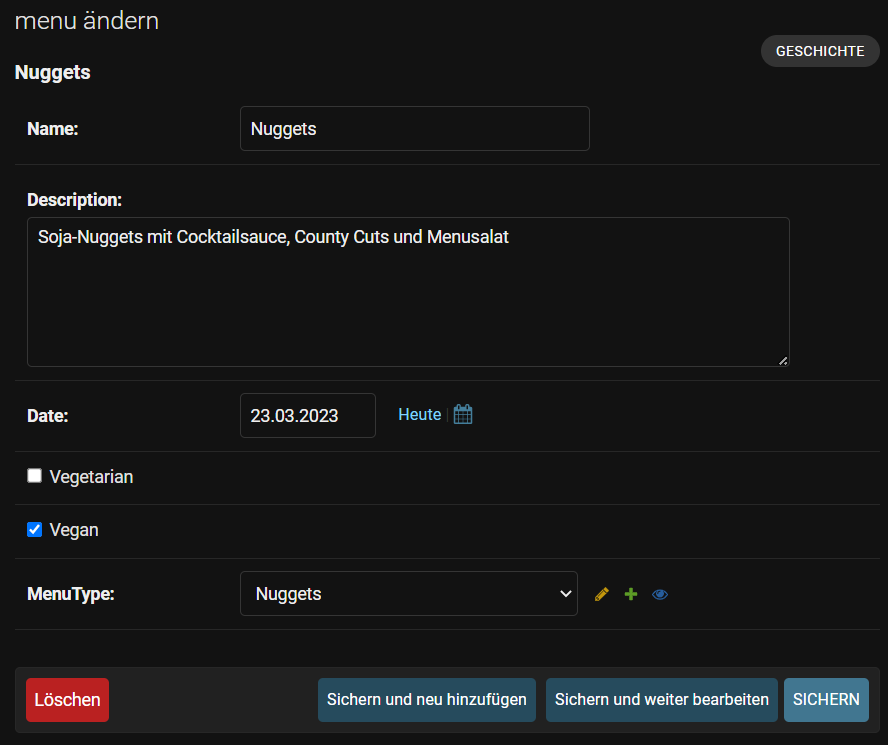
\includegraphics[width=0.7\textwidth]{images/Resultat-admin-menu.png}
        \caption{Screenshot: Spezifischer Menu Eintrag}
        \label{fig:r-adminpanel-menu}
    \end{subfigure}
    \hfill
\end{figure}


Auf dem bereitgestellten Admin Panel von Django (siehe \ref{fig:r-adminpanel})
können Administratoren Einträge in der Datenbank hinzufügen, löschen und
verändern.


